\documentclass[11pt,a4paper]{article}
\usepackage[T1]{fontenc}
\usepackage[utf8]{inputenc}
\usepackage{lmodern,microtype}
\usepackage[a4paper,margin=24mm,headheight=15pt]{geometry}
\usepackage{amsmath,amssymb,amsthm,mathtools,stmaryrd}
\usepackage{booktabs,longtable,tabularx,array,enumitem}
\usepackage{xcolor,listings,tcolorbox,tikz}
\usetikzlibrary{arrows.meta,positioning}
\usepackage{fancyhdr,needspace,xurl,etoolbox}
\usepackage[pdfusetitle,colorlinks=true,linkcolor=Juniper,citecolor=Juniper,urlcolor=Juniper]{hyperref}
\definecolor{Juniper}{HTML}{175B4E}
\definecolor{Pale}{HTML}{F1F6F3}
\definecolor{Ink}{HTML}{24332F}
\definecolor{RuleGray}{HTML}{D3DDD7}
\hypersetup{pdftitle={Juniper: Property-Directed Mathematics with Explicit Obligation Frontiers},pdfauthor={OpenAI, prepared for Vladimir Reshetnikov}}
\pagestyle{fancy}\fancyhf{}
\fancyhead[L]{\small\sffamily\color{Juniper} JUNIPER\quad /\quad ROUND FOUR}
\fancyhead[R]{\small\sffamily\thepage}
\renewcommand{\headrulewidth}{0.4pt}
\setlength{\parindent}{0pt}\setlength{\parskip}{0.52em}
\setlength{\emergencystretch}{2em}
\setcounter{tocdepth}{2}
\setlist{nosep,leftmargin=1.7em,topsep=0.4em}
\newcommand{\code}[1]{\texttt{\small\detokenize{#1}}}
\newcommand{\R}{\mathbb R}\newcommand{\Q}{\mathbb Q}\newcommand{\Z}{\mathbb Z}\newcommand{\N}{\mathbb N}
\newcommand{\Prop}{\mathsf{Prop}}\newcommand{\Cl}{\operatorname{Cl}}\newcommand{\Min}{\operatorname{Min}}
\newcommand{\Beh}{\operatorname{Beh}}\newcommand{\Req}{\operatorname{Req}}
\newcommand{\view}{\mathrel{\triangleright}}\newcommand{\supp}{\operatorname{supp}}
\newcommand{\floorc}[1]{\left\llbracket #1\right\rrbracket}
\newtheorem{theorem}{Theorem}[section]
\newtheorem{proposition}[theorem]{Proposition}
\newtheorem{lemma}[theorem]{Lemma}
\theoremstyle{definition}\newtheorem{definition}[theorem]{Definition}
\theoremstyle{remark}\newtheorem{remark}[theorem]{Remark}
\lstdefinestyle{juniper}{basicstyle=\ttfamily\small,backgroundcolor=\color{Pale},
  frame=single,rulecolor=\color{RuleGray},framesep=7pt,breaklines=true,
  columns=fullflexible,keepspaces=true,showstringspaces=false,
  aboveskip=0.8em,belowskip=0.7em,tabsize=2}
\lstset{style=juniper}
\BeforeBeginEnvironment{lstlisting}{\par\noindent\begin{minipage}{\linewidth}}
\AfterEndEnvironment{lstlisting}{\end{minipage}\par}
\newtcolorbox{principle}{colback=Pale,colframe=Juniper,boxrule=0.6pt,arc=1mm,left=3mm,right=3mm,top=2mm,bottom=2mm}
\newcolumntype{Y}{>{\raggedright\arraybackslash}X}
\newcolumntype{L}[1]{>{\raggedright\arraybackslash}p{#1}}
\title{Juniper: Property-Directed Mathematics with Explicit Obligation Frontiers}
\author{Prepared for Vladimir Reshetnikov}
\date{September 6, 2026}
\begin{document}
\begin{titlepage}
\color{Ink}
{\sffamily\small\color{Juniper} FOURTH-ROUND PROOF-LANGUAGE PROPOSAL}\par
\vspace{18mm}
{\sffamily\bfseries\fontsize{49}{54}\selectfont Juniper}\par
\vspace{6mm}
{\sffamily\Large Property-Directed Mathematics\par with Explicit Obligation Frontiers}\par
\vspace{8mm}
{\large A conservative extension of Lean's authoring discipline,\par with behavioral contracts and proof-producing computation}\par
\vspace{12mm}
\begin{principle}
\textbf{The central idea.} A mathematical step should say what the author intends to do. Juniper should infer the evidence that licenses that step, and expose a finite, proof-backed account of what remains missing. It must never obtain concision by silently changing the object, the hypotheses, or the claim.
\end{principle}
\vspace{7mm}
This article reads the two round-three syntheses together, checks representative source declarations in ProveIt, the FLT repository, and Leant, and develops a specific fourth-round increment: \emph{residual proof telescopes and a bounded antichain algorithm for alternative sufficient premise sets}.

The accompanying reference implementation parses a small ground propositional language, computes these frontiers, validates derivation graphs, and exports generic Lean implication proofs. The larger mathematical surface and the Lean integration remain designs, not implemented features.
\vfill
{\sffamily Prepared for Vladimir Reshetnikov\par September 6, 2026}\par
\vspace{4mm}
{\small Evidence status: paper proofs; executed Python reference and tests; uncompiled generated Lean. No productivity study or full repository build is claimed.}
\end{titlepage}

\section*{Abstract}
\addcontentsline{toc}{section}{Abstract}
Lean can already express remarkably rich mathematical specifications. The difficulty is often that their consequences must be repeatedly reconstructed at use sites: an identity on an open set becomes a neighborhood identity; a smoothness hypothesis licenses a chain rule at a point in a function's image; an integer quotient agrees with a rational quotient only after divisibility is established. Merely making tactic scripts less visible does not solve this interface problem.

Juniper is a proposed mathematical authoring layer in which types describe an object's carrier, its fixed structures, its established properties, and the behavior expected of operations. The extension is primarily to elaboration: a proof-backed property index and property-implicit arguments compile to ordinary Lean terms. There is no semantic subtyping inside definitional equality, no automatic change of structure, and no new logical axiom. A richer kernel refinement former is evaluated as a research option, not presumed necessary.

The distinctive proposal is to make unfinished reasoning precise. A step produces a residual telescope and a proof valid under exactly that telescope. In a finite grounded Horn fragment, an antichain algorithm computes every inclusion-minimal set of designated additional premises sufficient for the goal. The article proves soundness, termination, relative completeness, and schedule independence for the specified algorithm, explains the exponential worst case, and specifies a bounded grounding discipline. These frontiers are explanations and proof plans, not permissions to assume their leaves.

Worked studies cover the autonomous-derivative proof, non-vacuous Frey exact division, analytic inverse derivatives certified through differential polynomials, quotient descent, and behavior-directed synthesis. The companion passes 32 unit tests; 400 generated rule profiles agree with an independent exhaustive oracle on 2,800 goal frontiers and with reversed rule schedules. It also checks 189 admissible arithmetic fixtures and computes inverse-derivative polynomials through order six. These are finite implementation checks, not a formal verification of the implementation. The generated Lean file was not compiled in this environment.

\begingroup\small\setlength{\parskip}{0pt}
\tableofcontents
\endgroup
\clearpage

\section{The proposal in one page}
\label{sec:proposal}
\textbf{Juniper should extend the type system that an author interacts with, while initially leaving Lean's trusted type theory unchanged.} Its basic judgment is not simply ``this expression has type $A$,'' but ``this exact expression has carrier $A$, under these fixed structures, with these proved properties, and this use demands the following evidence.''

The object remains ordinary Lean data. A local assertion enriches an evidence index, not the object's identity. At an exported interface, the same information can be packaged in a subtype or a structure. A behavioral annotation is an ordinary proposition about a function, possibly involving several inputs, several outputs, other functions, measures, domains, or precision indices. It is not an unchecked label.

Juniper's authoring loop is:
\begin{center}
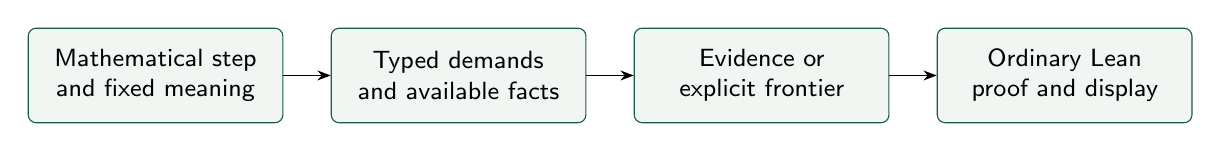
\begin{tikzpicture}[node distance=6mm, every node/.style={font=\small\sffamily,align=center},
box/.style={draw=Juniper,rounded corners=1mm,fill=Pale,minimum height=12mm,text width=30mm},
>=Stealth]
\node[box] (intent) {Mathematical step\\and fixed meaning};
\node[box,right=of intent] (demand) {Typed demands\\and available facts};
\node[box,right=of demand] (front) {Evidence or\\explicit frontier};
\node[box,right=of front] (proof) {Ordinary Lean\\proof and display};
\draw[->] (intent)--(demand);\draw[->] (demand)--(front);\draw[->] (front)--(proof);
\end{tikzpicture}
\end{center}

Three choices distinguish this proposal from a restatement of round three.
\begin{enumerate}
\item \textbf{Unfinished steps have a mathematical semantics.} Their output is a residual proof telescope, rather than a cache entry that looks like a proved fact. Dependent obligations and witness choices remain ordered.
\item \textbf{Alternative missing-premise explanations have an algorithm.} For an explicitly finite fragment, Juniper computes an antichain of sufficient premise sets and retains an acyclic derivation for each route. The advertised completeness is relative to that fragment and its designated premises, never to all of mathematics.
\item \textbf{The design is accompanied by a narrow executable slice.} A small parser, solver, derivation validator, and generic Lean exporter exercise the algorithm and failure states. They do not implement Lean's elaborator or pretend that symbolic atom names are mathematical theorems.
\end{enumerate}

The appropriate stopping condition is equally important. If the same improvement is obtained from a property library, existing tactics, and a better renderer, those should be the product. Juniper is justified only by additional, measured improvements in authoring, diagnosis, or maintenance.

\section{What the sources actually establish}
\label{sec:sources}
\subsection{The two syntheses should be read as a reconciled discussion}
\emph{From Properties to Proof Obligations} and \emph{Nine Refinements} converge on the same architecture: fixed objects, locally accumulated evidence, theorem-backed behavioral contracts, structure selection before property inference, bounded automation, and an unchanged initial kernel \cite{synA,synB}. The second report's revised discussion explicitly incorporates corrections from the first. Their overlapping conclusions therefore should not be counted as independent experimental evidence that a language works.

The most useful conclusion is also their most demanding one: another vocabulary for refinement rows is not the missing contribution. Neither report supplies an implemented general property-aware authoring interface. Their compilation work establishes that small semantic combinators can be expressed in ordinary Lean. That is valuable, but does not establish predictable elaboration, statement fidelity, or lower author effort.

Juniper adopts the following corrections, not the stronger claims that earlier drafts sometimes made:

\textbf{Sound finite certificates need not be complete.} A sound checker may prove every claim it accepts while rejecting some true claims. A negative abstract witness requires a realizability argument and a transfer premise before it refutes a concrete specification. These are different obligations.

\textbf{Equivalent designs are not identical encodings.} Local propositions, subtypes, and records can represent related interfaces without being alpha-equivalent Lean terms. Proof irrelevance concerns proofs of the same proposition, not distinct structures or arbitrary changes of carrier.

\textbf{A useful rule supplies sufficient premises.} The premises of one interchange theorem, one inverse theorem, or one least-Lipschitz-constant argument are not automatically mathematically necessary conditions. An obligation diagnostic should name its selected route.

\textbf{A proof checked in an inconsistent context does not test an arithmetic interface.} The Frey helper should be exercised under satisfiable arithmetic assumptions, not only under a full package eventually shown impossible.

\textbf{A statement can lose a premise during exposition.} The reports identify an omitted finite/free assumption in a reconstruction of a representing algebra. This is evidence for preserving exact signatures in the default mathematical view, not evidence that the original Lean theorem was wrong \cite{synA,synB}.

\subsection{Representative code, not a caricature of Lean}
The selected files expose several different costs. They also contain short proofs that Juniper should not make longer.

\begin{table}[htbp]\small
\caption{Source workloads examined. File names are abbreviated here; full paths and revisions are recorded in the source manifest.}
\begin{tabularx}{\textwidth}{@{}L{31mm}Y Y@{}}\toprule
Source & Mathematical work & Authoring issue to target\\\midrule
ProveIt, autonomous derivatives & Induction, neighborhood equality, chain rule & Preserve a set-wide induction hypothesis and infer the locality bridge.\\
ProveIt, inverse derivative recursion & Formal Bell coefficients and analytic differential operators & Do not promote a formal coefficient result into an analytic derivative theorem without a bridge.\\
FLT, Frey package and integer model map & Bundled assumptions, divisibility, casts, coefficient equality & Infer guards of exact quotient transport, independently for each coefficient.\\
Leant, verification and post-verification & Callback acceptance, exact candidate receipts, scoped reordering & Preserve identity and distinguish receipts from proof objects.\\
Leant, Length contracts & Explicit provider laws and source-ordered relational contracts & Attach denotation theorems to abstract behavior rather than interpreting names as semantics.\\\bottomrule
\end{tabularx}
\end{table}

The autonomous theorem in ProveIt already factors out a reusable mathematical argument. Its successor case obtains eventual equality from an identity throughout an open set and applies the chain rule. The wrapper for globally differentiable auxiliary functions is short \cite{ode}. The final FLT solution wrapper is also short; the larger file includes several reusable arithmetic and discriminant lemmas, not one enormous proof of the displayed final statement \cite{freyMap}. Whole-file line counts would be a misleading compression baseline.

The inverse-derivative file makes an unusually important distinction in its own documentation. Its Bell-polynomial recursion is established in a formal power-series setting; the analytic operator theorem is proved separately. The file explicitly does not claim an analytic Bell-form recursion or analytic third and fourth derivative formulas from those formal coefficient results alone \cite{inverse}. Juniper must preserve that separation even when the formulas look identical on the page.

\subsection{Existing Lean features are baselines, not Juniper inventions}
Lean's subtypes already bundle a value and a proof, and their compiled representation does not add a runtime wrapper. An argument for new kernel refinements cannot therefore rest on a blanket claim that ordinary subtypes necessarily cost runtime allocation \cite{leanSubtype,leanRuntime}. The real questions are elaboration effort, transports, proof-term size, and interface stability.

Mathlib's \code{fun_prop} already performs compositional property reasoning, uses registered theorems, and can discharge local side conditions. Its documentation also describes limits on transition-theorem chains because those chains enlarge search \cite{funprop}. Juniper must compare its property engine with this functionality, not with a baseline stripped of it. Lean's \code{grind} is another existing proof-producing service \cite{grind}. The \code{mvcgen} infrastructure already presents monadic programs through predicate transformers and verification conditions; round-three tests described it as experimental at their Lean 4.32.0 pin \cite{mvcgen,synA,synB}.

For historical orientation, bidirectional typing supplies the distinction between synthesizing information and checking against a demand; refinement-directed synthesis supplies a precedent for propagating specifications into program construction; Dijkstra monads supply a precedent for computing proof obligations from desired behavior \cite{bidir,synquid,dmfree}. Juniper's proposed contribution is their disciplined integration with mathematical locality, ordinary Lean evidence, and explicit alternative frontiers, not the invention of these ideas.

\section{What a mathematician would write}
\label{sec:surface}
All listings in this section are \textbf{proposed mathematical surface syntax}. They are not accepted by the companion parser. Section~\ref{sec:prototype} separately documents the implemented ground language.

\subsection{State the mathematical move, retain its scope}
A compact rendering of the autonomous-derivative argument could be:
\begin{lstlisting}
theorem autonomous_derivatives:
  given U : Set Real with Open U
  given W, phi : Real -> Real
  given G, Gprime : Nat -> Real -> Real
  assume derivative W at x is phi(W(x)) on U
  assume G(0, W(x)) = W(x) on U
  assume for every n:
    derivative G(n) at W(x) is Gprime(n, W(x)) on U
  assume for every n:
    G(n+1, W(x)) = Gprime(n, W(x))*phi(W(x)) on U
  prove for every n: D^n W = G(n) o W on U
  by induction n keeping the domain U:
    zero: use the initial identity
    step:
      differentiate the preceding identity on U
        using the chain rule
      use the recurrence
\end{lstlisting}
The first derivative assumption is an assertion of a derivative, translated to \code{HasDerivAt}, not merely an equation about Lean's total \code{deriv} operation. ``On $U$'' expands to a quantified predicate. ``Keeping the domain'' means that the induction hypothesis quantifies over every point of $U$ before the successor point is introduced. These are semantic choices that the compact view must preserve.

The phrase ``differentiate the preceding identity'' is a registered recipe. At a point $x\in U$ it requires eventual equality in $\mathcal N(x)$. A route from equality on $U$ requires $U\in\mathcal N(x)$; openness and membership are one sufficient way to obtain that premise. The author need not spell out the filter lemmas, but the elaborated proof must use them or another explicitly permitted route.

\subsection{Contracts at call sites}
An operation can expose a property-implicit argument:
\begin{lstlisting}
use cast_exact_integer_quotient(n, d)
  requires d divides n
  requires d != 0
  concludes cast(n /[Int] d) = cast(n) /[Rat] cast(d)
\end{lstlisting}
The operation is not a global reinterpretation of division. Integer division and rational division remain distinct. The two guards are sought in the local evidence index; a missing divisibility fact becomes an obligation. The library author writes the detailed theorem once. The user sees its mathematical interface at every use.

\subsection{An incomplete step should remain visibly incomplete}
Suppose $f=g$ on $U$ and $x\in U$, but no neighborhood fact is available. A diagnostic could read:
\begin{lstlisting}
Step: transport the derivative from f to g at x
Status: conditional; no theorem has been closed

Sufficient route 1: prove U is a neighborhood of x
Sufficient route 2: prove f and g agree near x directly

Open U would discharge route 1 using the known x in U.
No additional hypothesis has been added to the theorem.
\end{lstlisting}
An explanation can use a stronger recognizable premise such as openness, while retaining the exact required premise $U\in\mathcal N(x)$. A theorem may be true by a different route even when both displayed routes fail. ``No route in this profile'' is not ``false.''

\subsection{Construction is a separate act}
A command asking for a sorting function has two outputs to obtain:
\begin{lstlisting}
construct sort : List A -> List A
  satisfying for every xs:
    Permutation (sort xs) xs
    and Sorted order (sort xs)
\end{lstlisting}
First there must be a candidate function. Then there must be evidence of the exact universal specification for that function, under the fixed order. Tests may guide the search; a length law alone does not meet the specification. The source chooses whether executable code is required or a noncomputable existence witness is acceptable.

\section{A property-aware typing discipline}
\label{sec:types}
\subsection{Three environments, not one bag of hints}
Let $\Sigma$ be the selected mathematical signature: carrier types, universe parameters, operations, structures, and approved representation maps. Let $\Gamma$ be Lean's local context. Let $\mathcal E$ be an index of already checked evidence available in that context. A local view is written
\[
  \Sigma;\Gamma;\mathcal E\vdash t:A\view\{P_1(t),\ldots,P_k(t)\}.
\]
Every row entry has an actual proof in $\Gamma$. The index may accelerate finding that proof, but is not a second source of logical authority.

An anchor is a typed term in this context, including the instantiated data arguments that determine its meaning. Printed variable names are not anchors. Neither is a hash alone. For example, changing the topology changes the proposition \code{Continuous f}; changing a scalar action changes the proposition that a map is linear. Those changes cannot be hidden behind proof irrelevance.

The local introduction and consequence rules are intentionally ordinary:
\[
\frac{\Gamma\vdash t:A\quad\Gamma\vdash p:P(t)}
     {\Gamma\vdash t:A\view\{P\}},
\qquad
\frac{\Gamma\vdash p:P(t)\quad\Gamma\vdash h:P(t)\to Q(t)}
     {\Gamma\vdash t:A\view\{Q\}}.
\]
Conjunction combines proofs about the same anchor. Equality elimination transports a predicate along an actual equality. A weaker observational relation requires a theorem naming the property that the relation preserves. A pointwise equality, an almost-everywhere equality, and agreement of finitely many coefficients are not interchangeable labels.

\subsection{Local rows and exported types}
The local notation does not force rebinding $t$ to a subtype after every discovered fact. At a boundary, a package may be generated:
\[
 \{x:A\mid P_1(x)\land\cdots\land P_k(x)\}.
\]
A mixed interface containing witness data uses a dependent record instead. For instance, a chosen basis is data; finite-dimensionality is a proposition. A chosen inverse algorithm is data; the statement that an element is a unit is a proposition. Adding a proof-only row must not silently choose either witness.

This is a genuine extension of the \emph{surface typing discipline}: a call can be accepted by insertion of an inferred proof argument or a theorem-backed view adapter that plain use-site elaboration would not automatically discover. It is not an increase in what propositions Lean can express. The translation exposes every inserted argument and adapter as ordinary Lean terms.

\subsection{Property-implicit arguments}
A library operation can declare selected proof arguments as \code{requires} parameters. Its implementation is an ordinary dependent function with explicit proof binders. Juniper's call elaborator tries to fill those binders from available evidence and registered theorem recipes. It must not turn every discovered fact into a global type-class instance.

The proof search may create fresh local proof metavariables, but must not solve a meaning-bearing variable by changing a carrier, a branch, a quantified object, or a measure. Lean's synthetic opaque holes already distinguish certain deferred proof goals from ordinary inference holes; Juniper needs an additional audited staging policy, not a claim that all holes are currently indistinguishable \cite{leanHoles}.

The permissions should be explicit:
\begin{center}\small
\begin{tabularx}{\textwidth}{@{}L{29mm}Y Y@{}}\toprule
Hole class & What may be chosen & What remains fixed\\\midrule
Meaning inference & Ordinary elaboration resolves notation, structures, and indices before sealing. & The agreed mathematical statement after sealing.\\
Proof synthesis & A proof of an already fixed proposition. & Its proposition and the authorized context.\\
Construction & A value and evidence satisfying an explicitly delegated specification. & The specification, input domain, branch conditions, and execution requirement.\\\bottomrule
\end{tabularx}
\end{center}

A constructive witness hole can affect later expressions that explicitly depend on its result. That does not allow it to instantiate a universally quantified parameter of the original theorem. The distinction is an information-flow rule for elaboration, not a test based on whether a variable's printed name begins with a question mark.

\subsection{Proof irrelevance and dependent transport}
For the same proposition $P(t)$, different proof terms do not represent different mathematical objects. It does not follow that two structures on $A$ are identical, or that $\{x:A\mid P(x)\}$ and $\{x:A\mid Q(x)\}$ are definitionally equal merely because $P$ and $Q$ are logically equivalent.

A particularly revealing case is an indexed object $v:\operatorname{Vector}(A,n)$. If a proof establishes $n=m$, then a view of $v$ at index $m$ requires a dependent transport or a registered adapter; the fact that $n$ and $m$ happen to print similarly is irrelevant. Juniper should keep that transport in the evidence graph and explain it on demand, rather than requiring a new kernel conversion rule for every index identity.

\section{Residual telescopes: the meaning of an unfinished proof}
\label{sec:residual}
\subsection{From a missing premise to a conditional derivation}
An unfinished operation has the judgment
\[
 \Sigma;\Gamma;\mathcal E\vdash \mathsf{step}\Rightarrow(P,\Delta,k),
 \qquad \Gamma\vdash k:\Pi\Delta,\,P.
\]
Here $P$ is the locked target, $\Delta$ is a well-formed telescope of remaining obligations, and $k$ is a derivation that works when those obligations are supplied. The target may depend on the telescope's earlier binders where that dependency is explicitly part of the construction request. A completion supplies a well-typed substitution $\theta$ for every binder of $\Delta$; the resulting proof is $k\,\theta$.

For a proof-only residual,
\[
 \Delta=(h_1:P_1)(h_2:P_2)\cdots(h_r:P_r),
\]
this is simply a curried implication. The crucial rule is that $k$ is not inserted into the fact index as a proof of $P$ until its arguments exist. Juniper may store $k$ as a conditional plan, with a different type and a different user-visible status.

\subsection{Why a telescope is necessary}
Not every residual is a set of independent propositions. Constructing a quotient factorization can leave
\[
 (g:Y\to Z),\quad (h:g\circ q=f),\quad (c:\operatorname{Continuous}(g)).
\]
The last two items depend on the first. Flattening them into unrelated existential claims would permit the equation to concern one function and continuity another. Similarly, a root value, a branch-membership proof, and a residual-zero proof must refer to the same root.

Juniper therefore uses two levels. The general interface is a dependent telescope. The finite antichain engine of Section~\ref{sec:frontier} applies only after all data arguments relevant to its atoms are fixed. It neither invents witnesses nor pretends to solve dependent existential synthesis by propositional saturation.

\subsection{Residual composition}
Suppose a first recipe gives $k:\Pi\Delta, Q$ and a second, after receiving $q:Q$, gives $\ell:\Pi\Theta(q),P$. The composed residual retains the dependency:
\[
 \Pi\delta:\Delta,\ \Pi\eta:\Theta(k\delta),\ P.
\]
Its proof is $\lambda\delta\,\eta.\,\ell(k\delta)\eta$. One cannot discharge an item of $\Delta$ by appealing to $P$ unless an independent, well-founded proof supplies that item. This is the formal reason a result must not manufacture its own guard.

\begin{proposition}[Residual discharge]
If $\Gamma\vdash k:\Pi\Delta,P$ and $\Gamma\vdash\theta:\Delta$ is a valid dependent substitution, then $\Gamma\vdash k\theta:P$. Branch-local variables and proof assumptions cannot escape if the substitution is checked in $\Gamma$.
\end{proposition}
\begin{proof}
Apply the dependent function successively to the terms of $\theta$, in telescope order. Each application has the type obtained by substituting the preceding arguments. The final type is $P$ with the same authorized substitution. No free variable outside $\Gamma$ can appear in a well-typed argument supplied by $\theta$.
\end{proof}

This elementary proposition does not verify an implementation of elaboration. Its purpose is to make the required implementation invariant explicit: an open residual is not a theorem, and completion is checked substitution rather than a change of status in a database.

\subsection{Drafts, assertions, and publication}
An author may keep a draft with open residuals. Publication as a verified theorem requires closure of the theorem and every displayed assertion presented as established, even an assertion unused in the final proof. Otherwise an attractive narrative could contain false intermediate claims beside a correct terminal theorem.

The renderer should distinguish an assumption made in the theorem statement, a locally assumed case, a proved assertion, a conditional plan, and an informal comment. Collapsing these into the same typography would defeat the entire design. Conditions changing the claim belong in the default view, not solely in a hover panel.

\section{A bounded algorithm for alternative obligations}
\label{sec:frontier}
\subsection{The finite problem}
Trellis already gives a finite qualifier-closure theorem, and the two syntheses ask for a bounded rule generator and an effective obligation frontier \cite{trellis,synA,synB}. Juniper extends that specific finite problem from \emph{available facts} to \emph{alternative sufficient additions}. The set-theoretic machinery is not claimed as a new foundation of logic; its role here is to make the proposed authoring contract exact and testable.

Fix a finite set $A$ of grounded atoms, a set $K\subseteq A$ of known facts, a set $H\subseteq A$ of designated additional premises, and a finite collection $R$ of rules
\[
 r:\quad a_1\land\cdots\land a_k\longrightarrow b.
\]
A ground atom can contain an arbitrary local variable, provided its data arguments and context are fixed. Thus $x\ne0$ with a local $x:\R$ is ground for this purpose; no enumeration of real numbers is involved. Each actual mathematical rule must be an instantiated Lean theorem. A rule with no premises is an available theorem.

Let $\Cl_R(X)$ be ordinary forward Horn closure from $X$. Define the frontier of $b$ by
\begin{equation}\label{eq:frontier}
 \mathcal F(b)=\Min_{\subseteq}\{S\subseteq H\mid b\in\Cl_R(K\cup S)\}.
\end{equation}
Only inclusion-minimal sets are retained. The empty set means no additional premise is needed. An empty \emph{family} means no permitted set of additions suffices in this rule system. These cases must never share the same representation in an implementation.

$H$ is a diagnostic vocabulary, not a new assumption context. A member may be a proposition the author could prove, an explicit premise the author is considering adding, or a currently open named obligation. The default interface should not offer the goal itself as a helpful repair. The mathematical definition permits that case when explicitly requested: its result is a conditional tautological route, not a proof.

\subsection{Antichain propagation}
For each $a\in A$, maintain an antichain $F(a)$ and a derivation node for every stored support. Initialize
\[
 F(a)\supseteq\{\varnothing\}\ (a\in K),\qquad
 F(h)\supseteq\{\{h\}\}\ (h\in H),
\]
then remove dominated sets. For every rule $a_1,\ldots,a_k\to b$ and every tuple $S_i\in F(a_i)$, form $S=\bigcup_i S_i$. Insert $S$ into $F(b)$ unless an existing support is contained in $S$; on insertion remove strict supersets of $S$. Repeat until there is no change.

A newly inserted derivation node contains the instantiated rule and references to \emph{already existing} premise nodes. It never points to a placeholder for its own conclusion. A removed antichain entry's node may remain in the derivation store if later nodes reference it. This preserves valid proof sharing while the presentation keeps only minimal supports.

\Needspace{17\baselineskip}
\begin{lstlisting}
frontier[known_atom] += { empty_support }
frontier[offered_atom] += { singleton(offered_atom) }
repeat:
  changed := false
  for each ground rule premises -> conclusion:
    for each tuple of currently available premise supports:
      support := union(tuple)
      if no stored support is a subset of support:
        retain a node referring only to older premise nodes
        remove strict supersets; insert support
        changed := true
until not changed
\end{lstlisting}

\subsection{Soundness and termination}
\begin{theorem}[Sound conditional derivations]\label{thm:sound}
Every stored entry $S\in F(b)$ admits a finite derivation of $b$ from $K\cup S$ using $R$. Under an interpretation of the atoms as Lean propositions and of the rules as checked theorem instances, its derivation yields a proof of $b$ under the corresponding explicit premises.
\end{theorem}
\begin{proof}
Induct on node creation order. A known node uses its proof from $K$ and has empty additional support. An offered node uses its corresponding premise and has singleton support. For a rule node, the induction hypotheses provide proofs of each premise under its recorded support. Under their union, all those proofs are available by weakening. Apply the instantiated rule theorem. All parent nodes precede the new node, so this argument is well-founded even when the rule graph contains cycles. Deleting a dominated display entry does not invalidate its retained node or any later use of that node.
\end{proof}

Antichains themselves are not monotone under ordinary set inclusion: a smaller support can replace a larger one. The right termination measure uses upward closures. For a family $F\subseteq\mathcal P(H)$, put
\[
 \uparrow F=\{S\subseteq H\mid\exists T\in F,\ T\subseteq S\}.
\]
\begin{theorem}[Finite convergence]\label{thm:terminate}
Every accepted insertion strictly enlarges one upward closure $\uparrow F(a)$. Consequently there are at most $|A|2^{|H|}$ accepted insertions, including initialization, and a full-sweep implementation terminates.
\end{theorem}
\begin{proof}
An insertion of $S$ is rejected whenever some existing $T\subseteq S$ exists. If accepted, $S$ was not in the old upward closure and is in the new one. Removing strict supersets loses no element of the upward closure because $S$ covers all of them. Thus the upward closures increase monotonically, and each accepted insertion adds at least one pair $(a,S)$ from a set of size $|A|2^{|H|}$. Between insertions a sweep visits finitely many rules and finite products of support families. A sweep without an insertion halts the algorithm.
\end{proof}

The $|A|$ bound for ordinary fact closure does \emph{not} carry over to support propagation. The extra exponential factor is real and should be part of the interface contract.

\Needspace{8\baselineskip}
\subsection{Relative completeness and schedule independence}
\begin{theorem}[Exact minimal frontier]\label{thm:complete}
At a fixed point, $F(b)=\mathcal F(b)$ for every $b\in A$. Any fair rule schedule that eventually processes enabled support combinations obtains the same antichains, though its derivation graphs may differ.
\end{theorem}
\begin{proof}
Soundness shows that every stored support is sufficient. For the other direction, suppose $b\in\Cl_R(K\cup S)$. Induct on a finite Horn derivation of this fact. A known leaf is covered by the empty support. An offered leaf in $S$ is covered by its singleton or by a smaller stored support. At a rule application, each premise has a stored support $T_i\subseteq S$ by induction. At a fixed point the union $\bigcup_i T_i$ is covered by some support $T\in F(b)$, so $T\subseteq S$.

Therefore every sufficient $S$ contains a stored sufficient support. If $S$ is inclusion-minimal, that support equals $S$. Conversely, if a stored support were not minimal, a smaller sufficient set would contain another stored support and contradict the antichain condition. This proves equality. Fairness ensures that a terminal state has the same closure property; the uniquely specified family in~\eqref{eq:frontier} then gives schedule independence.
\end{proof}

The theorem is deliberately relative. It says nothing about omitted theorem instances, unoffered premises, a stronger semantic equivalence between offered propositions, or mathematical arguments outside $R$. ``Minimal'' does not mean a globally weakest hypothesis, the smallest number of words, or the fastest proof.

\subsection{A checkable completeness certificate}
A frontier producer should not be trusted merely because it returns a flag saying ``complete.'' There is a useful finite certificate characterization.

\begin{theorem}[Frontier certification]\label{thm:cert}
An antichain family $F$ is the exact frontier if the following conditions hold:
\begin{enumerate}
\item every displayed support has a valid finite derivation from its support and $K$;
\item every $a\in K$ is covered by the empty support, and every $h\in H$ is covered by $\{h\}$;
\item for every rule $a_1,\ldots,a_k\to b$ and tuple $S_i\in F(a_i)$, some $T\in F(b)$ satisfies $T\subseteq\bigcup_i S_i$.
\end{enumerate}
\end{theorem}
\begin{proof}
Condition 1 implies soundness of every upward-closed family $\uparrow F(a)$. Conditions 2 and 3 make those families a rule-closed over-approximation of all seed supports. Induction on any finite Horn derivation therefore shows that every sufficient support is covered. Soundness and coverage give equality with the sufficient-support families; taking their minimal members gives~\eqref{eq:frontier}.
\end{proof}

The companion's independent validator checks these conditions when a result is marked complete. For a budget-interrupted result it checks only the derivations and the current antichains. Such a result may contain useful sufficient routes, but does not claim global minimality or coverage even within the complete profile. This distinction is testable by deleting one alternative route or falsely setting a truncated result's completion flag.

This certificate theorem is a paper theorem about a finite representation. The Python validator is not a formally verified checker, and the current Lean exporter does not certify frontier completeness in Lean. A small Lean implementation of this checker is a concrete next deliverable, more specific than another generic statement that a future elaborator should be sound.

\subsection{Example and cost}
Take known facts \code{OnSet}, \code{Member}, and offered premises \code{Open}, \code{DirectGerm}, \code{Positive}. Rules derive a germ from either the open-set route or direct evidence, derivative equality from the germ, nonzeroness from positivity, and a quotient step from both. The frontier is
\[
 \{\{\mathsf{Open},\mathsf{Positive}\},
    \{\mathsf{DirectGerm},\mathsf{Positive}\}\}.
\]
The prototype produces precisely these two supports. They do not say that openness or positivity is necessary in analysis. They say that these are the minimal sufficient \emph{offered} combinations for these registered routes.

The exponential case is not pathological bookkeeping. Give each of $k$ independent intermediate facts two alternative offered premises and make the goal require all $k$ facts. There are $2^k$ pairwise incomparable sufficient sets. No algorithm explicitly listing every route can avoid output proportional to that number. An interactive system should normally display a small ranked selection and expose whether enumeration is complete. A bounded top-$k$ display and an exact all-routes certificate are different products.

Finally, support size does not determine proof cost. Two routes with the same support may have very different terms or runtimes. Version one retains one derivation per support and makes no optimality claim. Later versions may retain a bounded Pareto set for support, proof size, and recipe policy, but their guarantees need separate statements.

\section{Grounding rules without unbounded search}
\label{sec:grounding}
\subsection{A finite automatic fragment must say how it becomes finite}
The syntactic Horn calculus does not itself solve the difficult task of selecting useful Lean theorem instances. Juniper proposes a staged, bounded generator, not a universal principal-refinement algorithm.

At the beginning of a step, the elaborator records a finite term pool $T_0$ consisting of the target's typed subterms, relevant local declarations, and explicitly selected recipe parameters. Structures and universe arguments that determine propositions are resolved at this stage. A registry entry declares a conclusion pattern, its proof premises, data-input positions, and a bounded generation policy.

A conservative initial policy allows only data substitutions from a finite typed pool $T$. Recipe-specific constructors may extend the pool to depth $d$ and total size $B$, with both limits explicit. A theorem that would require a new function, basis, or inverse witness creates a construction residual; it does not cause saturation to enumerate arbitrary Lean terms. Repeated generation of $f(x),f(f(x)),\ldots$ therefore cannot continue without bound.

For a registry of $m$ entries with at most $k$ enumerable data positions, there are at most $m|T|^k$ raw assignments before typing and matching filters, when the pool is fixed. This is only a combinatorial bound on that specified enumeration. It excludes higher-order matching, reduction, instance resolution, checking proof arguments, and dependent well-formedness. Each successful assignment must yield a fully typed rule instance whose conclusion and premises are added to a finite manifest.

\subsection{Two completeness flags}
The front-end needs at least two separate indicators: \emph{grounding coverage within the selected policy} and \emph{frontier closure for the emitted manifest}. The frontier can be exact for the actual manifest even when the generator stopped before enumerating every permitted assignment. Reporting only the second flag would make a partial mathematical search look complete.

The first implementation should favor explicitly registered, first-order-shaped theorem families and recipe-defined instantiations. Higher-order goals can be sent to ordinary Lean tactics or a synthesis service as a separate bounded action. A returned proof may seed a new snapshot; failure means only that the action did not return a proof.

The registry is not allowed to assert that a theorem instance exists merely because its name resembles a familiar lemma. Registering an entry checks its telescope, argument roles, target predicate, and selected structures. For external providers, the binding to the exact provider term is part of that check.

\subsection{Demand-directed closure}
After grounding, construct the backward dependency graph from the requested atom, retaining all premises of each retained rule. Saturating this closed subgraph preserves the exact frontier for the retained manifest. Heuristically dropping a rule may be a useful search optimization, but changes that manifest and must be reported as such.

Unknown facts should not trigger an indiscriminate search through the entire environment. A method can first ask for a narrowly targeted property: nonzeroness at a specified point, membership in a chosen domain, eventual equality at a specified filter, or the exact division law for a particular numerator and denominator. This is the operational meaning of property-directed authoring.

\subsection{Scope and rewriting}
Version one rebuilds the index at branch boundaries and after relevant edits. This costs more than an ideal persistent engine but gives a tractable correctness boundary. Parent facts can be reused in a child only through a valid context embedding. Reusing a fact in a sibling or after a deleted assumption is not permitted because the variable names still match.

A simplification from $t$ to $u$ has three possibilities: definitional conversion, an actual equality proof with transport, or a registered relation appropriate to the consumer. The old property is not silently rebound to $u$. A proof of $f=g$ almost everywhere can serve a compatible integral consumer; it cannot authorize arbitrary pointwise evaluation.

An implementation may hash the signature and context to route lookups and reject stale data quickly. The hash is not a mathematical proof of context equivalence. General reuse after an edit ultimately requires rechecking the term in the new context or checking a typed substitution. The prototype demonstrates only exact-profile rejection, not full Lean context transport.

\section{Behavioral types beyond unary predicates}
\label{sec:behavior}
\subsection{Total functions and restricted-domain functions differ}
For a fixed total function $f:A\to B$, define
\[
 \Beh(f;P,Q):=\forall x:A,\ P(x)\to Q(x,f(x)).
\]
This is evidence about an already chosen total function. It is not generally the same object as a function defined only on a refined domain:
\[
 g:\Pi x:\{a:A\mid P(a)\},\ \{b:B\mid Q(x.\mathrm{val},b)\}.
\]
In particular, extending $g$ to all of $A$ may need extra data, decidability, or a default value. Juniper should use different surface constructs for a total function with a guarded law and for a function whose actual input is a subtype. It should not promise a total implementation by erasing a domain restriction.

\subsection{Variance with a proof, not a slogan}
\begin{proposition}[Behavioral weakening]
Suppose $\Beh(f;P,Q)$, $P'(x)\to P(x)$ for every $x$, and
\[
 P'(x)\to Q(x,y)\to Q'(x,y)
\]
for every $x,y$. Then $\Beh(f;P',Q')$.
\end{proposition}
\begin{proof}
Given $P'(x)$, obtain $P(x)$ and hence $Q(x,f(x))$. Apply the postcondition implication at the same $x$ and the actual output $f(x)$. Abstract over $x$ and its premise.
\end{proof}
The direction expresses contravariance of admissible inputs and covariance of promised outputs. The proof does not replace the implementation $f$. Juniper's subtyping-like behavior is insertion of this proof, not a new equality between function types.

\begin{proposition}[Composition with the actual intermediate value]
Suppose $\Beh(f;P,Q)$, $\Beh(g;S,T)$, and
\[
 \forall x,y,\ P(x)\to Q(x,y)\to S(y).
\]
Then $g\circ f$ satisfies
\[
 \forall x,\ P(x)\to
 Q(x,f(x))\land T(f(x),g(f(x))).
\]
\end{proposition}
\begin{proof}
Use the first contract to obtain $Q(x,f(x))$. The bridge supplies $S(f(x))$, so the second contract gives $T(f(x),g(f(x)))$. Pair the conclusions. No existentially chosen surrogate intermediate value is used.
\end{proof}

\subsection{Whole-function and relational contracts}
Monotonicity compares two inputs; additivity relates three evaluations; continuity quantifies over neighborhoods; naturality relates a family of maps; exactness concerns a diagram. Juniper's behavioral annotations must therefore admit arbitrary ordinary Lean predicates on these objects, not just a fixed menu of scalar input/output relations.

For example, a pair-valued partition operation can carry
\[
 \operatorname{Permutation}(\operatorname{left}(x){+\!+}\operatorname{right}(x),x),
\]
and joint membership conditions. Separate length bounds for the two outputs do not establish their combined content. Leant already has an explicit binary-product Length-contract vocabulary; Juniper should build on the source-ordered joint interface rather than reverting to independent output annotations \cite{lengthContract}.

For a representation map $v:A\to B$, \emph{preservation} of a relation and \emph{reflection} of it are different contracts:
\[
 R_A(x,y)\to R_B(vx,vy),\qquad
 R_B(vx,vy)\to R_A(x,y).
\]
A ring homomorphism preserves polynomial equality. Even an injective homomorphism need not reflect ideal membership after a change of coefficient domain. For example, $X$ belongs to the ideal generated by $2X$ in $\Q[X]$, using multiplier $1/2$, but not in $\Z[X]$, since comparison of the coefficient of $X$ would require an integer $c$ with $2c=1$. The operation's type must name which relation it transports.

\subsection{Behavioral abstractions and negative evidence}
Suppose an abstraction $\alpha:X\to D$ and a provider model $F:D\to D'$ satisfy
\[
 \beta(f(x))=F(\alpha(x)).
\]
A proof of an abstract specification may transfer positively through this equation. A counterexample $d\in D$ is different: one must obtain an admissible $x$ with $\alpha(x)=d$, and show that the abstract failure implies the concrete specification fails on that $x$.

The length abstraction makes the distinction vivid.
\begin{proposition}[The image of list length]
For a type $A$, a natural number $n$ is the length of a list over $A$ exactly when $n=0$ or $A$ is inhabited.
\end{proposition}
\begin{proof}
The empty list realizes zero. If $a:A$ exists, the list repeating $a$ exactly $n$ times realizes any $n$. Conversely, a nonempty list has a head, which witnesses that $A$ is inhabited. A list of positive length is nonempty.
\end{proof}
Thus an empty-output function on \code{List Empty} preserves every realizable input length, even though the abstract formula $0=n$ fails at positive natural numbers. Positive length is not a concrete counterexample in that domain.

For affine length models $an+b$ and $cn+d$ with $a,b,c,d\in\N$, equality on all realizable lengths reduces to $b=d$ when $A$ is empty, and to $a=c$ and $b=d$ when $A$ is inhabited. In the inhabited case evaluate at zero and one, then cancel the equal constants; the converse is substitution. This is a complete criterion for that abstraction and domain, not a free theorem for arbitrary polymorphic Lean programs.

A failed candidate refutes that candidate only. Pruning an entire partially specified program requires a proof that every permitted completion violates the demand, or an explicit label that the pruning is heuristic. Juniper should preserve this distinction at the synthesis boundary.

\section{Case study: exact arithmetic in the Frey model}
\label{sec:frey}
\subsection{The source already contains a property-rich object}
The FLT source defines a \code{FreyPackage} containing integers $a,b,c$, an exponent $p$, nonzeroness, primality and a lower bound, a Fermat equation, a gcd condition, and congruences. Its integral and rational Weierstrass models use visually parallel coefficient expressions \cite{freyDef}. The map theorem proves that their meanings agree by proving the necessary divisibility before transporting integer division \cite{freyMap}.

This is not an example of Lean being unable to express mathematical properties. It is an example of evidence already present in a rich package being reconstructed for a downstream operation. Juniper's potential improvement is at the operation boundary.

\subsection{Extract a satisfiable arithmetic interface}
Consider the helper context
\begin{equation}\label{eq:freycontext}
 a,b\in\Z,\qquad p\in\N,\qquad
 a\equiv3\pmod4,\quad 2\mid b,\quad p\text{ odd},\quad p\ge4.
\end{equation}
It is inhabited, for instance by $(a,b,p)=(3,2,5)$. It does not contain the Fermat equation, primality, or the gcd assumptions. Set
\[
 N_2=b^p-1-a^p,\qquad N_4=-a^pb^p.
\]
\begin{proposition}[Operation-specific divisibility]\label{prop:frey}
If $a\equiv3\pmod4$, $2\mid b$, $p$ is odd, and $p\ge2$, then $4\mid N_2$. Independently, if $2\mid b$ and $p\ge4$, then $16\mid N_4$.
\end{proposition}
\begin{proof}
Write $b=2k$. For $p\ge2$, $b^p$ is divisible by $4$. Since $a\equiv-1\pmod4$ and $p$ is odd, $a^p\equiv-1\pmod4$. Therefore $N_2\equiv0-1-(-1)=0\pmod4$.

For $p\ge4$, the factor $b^p=2^pk^p$ is divisible by $16$. Its multiple $-a^pb^p$ is consequently divisible by $16$, without any hypothesis on the residue of $a$ or the parity of $p$.
\end{proof}
The separate interfaces are stronger engineering choices than giving both operations the entire package. In particular, $(3,2,3)$ is admissible for the first quotient but not the second. This is a simple example of meaningful premise minimization that the library author can prove before any automatic frontier search.

\subsection{Exact quotient evidence}
Use a relation
\[
 \operatorname{ExactQuot}(n,d,q):\quad dq=n.
\]
Existence of such a $q$ is divisibility. Uniqueness in $\Z$ additionally requires $d\ne0$. To conclude that its image in $\Q$ is $n/d$, apply the homomorphism to $dq=n$ and divide by the nonzero image of $d$. These are distinct steps: preservation of the balance equation by a ring homomorphism is weaker than availability of division in the target.

For an arbitrary target ring, the appropriate condition is invertibility of the image of $d$, not merely its nonzeroness. A nonzero element need not be a unit; $2\in\Z$ is the elementary counterexample. A regular element licenses cancellation but still need not have an inverse. Juniper should not collapse the three predicates into one ``safe denominator'' flag.

Under~\eqref{eq:freycontext}, the two quotients at $(3,2,5)$ are $-53$ and $-486$. These values are finite sanity checks; Proposition~\ref{prop:frey}, not the examples, proves the general divisibility.

\subsection{A compact authoring sketch and its frontier}
\begin{lstlisting}
within integers and the selected embedding Int -> Rat:
  derive q2 := exact quotient (b^p - 1 - a^p) by 4
  derive q4 := exact quotient (-a^p * b^p) by 16
  transport both coefficients to Rat by exact quotient laws
  conclude equality of the Weierstrass models by coefficients
\end{lstlisting}
The source can preserve the already defined integer quotients as anchors rather than creating unrelated witnesses $q_2,q_4$. A recipe either proves their balance equations or explicitly constructs a new quotient and proves equality with the source definition.

A useful frontier records the separate paths: the first coefficient depends on a mod-$4$ power argument; the second depends on the exponent lower bound. It should not silently use a terminal contradiction about the full Frey package. A named arithmetic recipe can restrict the ground manifest to the intended arithmetic theorems. That is a reproducibility constraint on the elaboration recipe, not a theorem that the resulting proof ``essentially'' uses only one mathematical idea.

\begin{table}[htbp]\small
\caption{Boundary fixtures. Nonzero residues exhibit failure of the corresponding divisibility claim.}
\begin{tabularx}{\textwidth}{@{}L{26mm}Yrr@{}}\toprule
$(a,b,p)$ & Changed condition & $N_2\bmod4$ & $N_4\bmod16$\\\midrule
$(3,2,5)$ & Positive fixture & 0 & 0\\
$(3,2,4)$ & Exponent not odd & 2 & 0\\
$(3,3,5)$ & $b$ not even & 3 & 7\\
$(3,2,3)$ & Bound for the second quotient removed & 0 & 8\\
$(1,2,5)$ & Wrong residue of $a$ & 2 & 0\\\bottomrule
\end{tabularx}
\end{table}
These checks are under a satisfiable helper context. There is no need to manufacture a full Frey package to validate an arithmetic rule.

\section{Case study: analytic inverse derivatives with certified algebra}
\label{sec:inverse}
\subsection{A full mathematical contract}
Let $U,V\subseteq\R$ be open, $f:\R\to\R$ be smooth on $U$, and $g:\R\to\R$ be continuous on $V$. Assume
\begin{equation}\label{eq:inversecontract}
 g(V)\subseteq U,\qquad f(g(y))=y\quad(y\in V),\qquad
 f'(x)\ne0\quad(x\in U).
\end{equation}
This matches the shape of the analytic operator result in the examined ProveIt file \cite{inverse}. It fixes the inverse branch through the actual function $g$ and its local right-inverse law. Neither a formal series inverse nor an unspecified inverse notation is substituted for $g$.

\begin{lemma}[First inverse derivative]
Under~\eqref{eq:inversecontract}, $g$ is differentiable at every $y\in V$ and
\[
 g'(y)=\frac1{f'(g(y))}.
\]
\end{lemma}
\begin{proof}
Fix $y_0\in V$ and write $x_0=g(y_0)$. For $y$ near $y_0$ within $V$, continuity gives $g(y)\to x_0$. If $y\ne y_0$, the right-inverse identity implies $g(y)\ne x_0$. Hence
\[
 \frac{g(y)-g(y_0)}{y-y_0}
 =\left(\frac{f(g(y))-f(x_0)}{g(y)-x_0}\right)^{-1}.
\]
The inner quotient tends to $f'(x_0)$ by differentiability of $f$, and that limit is nonzero. Continuity of inversion at a nonzero real therefore gives the claimed limit. Openness of $V$ makes this an ordinary two-sided derivative at $y_0$, rather than a derivative restricted to an unspecified subset.
\end{proof}

The source's autonomous theorem provides the reusable mechanism for higher derivatives. A family $G_n$ with $G_0(x)=x$ and $G_{n+1}=G_n'/f'$ gives $g^{(n)}=G_n\circ g$. The proof differentiates an identity valid throughout the open set $V$, not just at the current point \cite{ode,inverse}.

\subsection{A differential-polynomial recurrence}
Let $u_j$ denote a formal variable corresponding to $f^{(j)}$. On the polynomial ring in the variables $u_1,u_2,\ldots$ over $\Z$, define the derivation
\[
 D(u_j)=u_{j+1},\qquad
 D(P)=\sum_{j\ge1}u_{j+1}\frac{\partial P}{\partial u_j}.
\]
Each polynomial involves only finitely many variables, so the displayed sum is finite. Define
\begin{equation}\label{eq:P}
 P_1=1,\qquad
 P_{n+1}=u_1D(P_n)-(2n-1)u_2P_n\quad(n\ge1).
\end{equation}

\begin{theorem}[Inverse derivatives from differential polynomials]\label{thm:inversepoly}
Under~\eqref{eq:inversecontract}, for every $n\ge1$ and $y\in V$,
\begin{equation}\label{eq:inverseformula}
 g^{(n)}(y)=
 \frac{P_n(f'(g(y)),f''(g(y)),\ldots,f^{(n)}(g(y)))}
      {f'(g(y))^{2n-1}}.
\end{equation}
\end{theorem}
\begin{proof}
For a polynomial $P$, ordinary differentiation and the chain and product rules give
\[
 \frac{d}{dx}P(f'(x),f''(x),\ldots)
       =(DP)(f'(x),f''(x),\ldots).
\]
One can prove this identity structurally for constants, variables, addition, and multiplication. This is the semantic theorem required of a differential-polynomial reifier.

Set
\[
 R_n(x)=\frac{P_n(f'(x),\ldots,f^{(n)}(x))}{f'(x)^{2n-1}}
 \quad(x\in U).
\]
Smoothness and nonzeroness of $f'$ imply that these expressions are differentiable on $U$. The quotient rule and~\eqref{eq:P} yield
\begin{align*}
 \frac{R_n'(x)}{f'(x)}
 &=\frac{f'(x)(DP_n)(f'(x),\ldots)
       -(2n-1)f''(x)P_n(f'(x),\ldots)}{f'(x)^{2n+1}}\\
 &=R_{n+1}(x).
\end{align*}
The first-derivative lemma establishes $g'=R_1\circ g$. If $g^{(n)}=R_n\circ g$ throughout $V$, differentiating at any point in $V$ gives
\[
 g^{(n+1)}=(R_n'\circ g)g'
           =(R_n'/f')\circ g=R_{n+1}\circ g.
\]
The identity being differentiated is local on an open set, and $g(V)\subseteq U$ licenses each occurrence of the guard. Induction proves~\eqref{eq:inverseformula}.
\end{proof}

This is a paper-level analytic derivation included here, not a claim that the examined repository already contains a kernel-checked theorem with this exact statement. It also does not follow merely from displaying the same formulas for formal Taylor coefficients. The analytic interpretation, the local inverse argument, and the quotient guards do the missing work.

\subsection{The first formulas and checkable invariants}
The recurrence gives
\begin{align*}
 P_1&=1,\qquad P_2=-u_2,\\
 P_3&=3u_2^2-u_1u_3,\\
 P_4&=-15u_2^3+10u_1u_2u_3-u_1^2u_4.
\end{align*}
Substitution in~\eqref{eq:inverseformula} yields the familiar first four inverse derivatives with their analytic hypotheses intact. The companion computes through $P_6$, using exact integer coefficients.

\begin{proposition}[Structural invariants of the polynomial family]
For $n\ge1$, every monomial of $P_n$ has ordinary degree $n-1$ and weighted degree $2n-2$ when $u_j$ has weight $j$. The polynomial involves no variable beyond $u_n$. The coefficient of $u_2^{n-1}$ is
\[
 (-1)^{n-1}(2n-3)!!,
\]
with $(-1)!!=1$. For $n\ge2$, the coefficient of $u_1^{n-2}u_n$ is $-1$.
\end{proposition}
\begin{proof}
The assertions about degree, weighted degree, and largest index hold for $P_1$. The derivation $D$ preserves ordinary degree, raises weighted degree by one, and raises the largest possible index by at most one. Multiplication by $u_1$ then raises ordinary degree by one and weighted degree by another one. Multiplication by $u_2$ in the second term of~\eqref{eq:P} has the same degree effects. Induction proves the three invariants.

The first term of~\eqref{eq:P} is divisible by $u_1$ and cannot contribute to a pure power of $u_2$. Its coefficient is therefore multiplied by $-(2n-1)$ at each step, starting from $1$ at $n=1$, giving the double factorial.

For $n\ge2$, the degree invariants show that a monomial involving $u_n$ can only be $u_1^{n-2}u_n$: using $u_n$ consumes weight $n$, and the remaining $n-2$ factors must each have the minimum weight one. In the recurrence the only contribution to $u_1^{n-1}u_{n+1}$ comes from differentiating this $u_n$ factor and multiplying by $u_1$. Its coefficient is inherited unchanged from $P_n$. The initial coefficient in $P_2=-u_2$ is $-1$.
\end{proof}

These invariants are useful contracts for a symbolic backend. They detect some errors cheaply, but do not certify an entire polynomial identity by themselves: a wrong coefficient can preserve both degrees. The proof-producing polynomial comparison still has to check the actual expression.

\subsection{How Juniper would factor the work}
\begin{lstlisting}
family inverse_derivative_formula(n) for n >= 1:
  use the fixed local inverse g of f from V into U
  retain f' nonzero on U
  define P by the differential-polynomial recurrence
  prove D^n g = (P(n)[derivatives f] / (f')^(2*n-1)) o g
    by induction using the inverse derivative rule

specialize n = 4
  normalize the polynomial certificate
\end{lstlisting}
The mathematical insight is the recurrence and the inverse branch. The analytic library proves the semantic derivative and locality rules. The symbolic backend expands or normalizes $P_n$. The property layer obtains $f'(g(y))\ne0$ from the already recorded map-into-domain and nonvanishing contracts whenever needed. The source author does not repeatedly reconstruct that implication.

A fixed-order polynomial calculation is a good CAS task. An arbitrary-order theorem is not proved by checking six examples; it uses the induction above or its formal counterpart. Juniper's interface should make that distinction explicit.

\subsection{Negative neighbors}
For $f(x)=x^3$, the inverse is continuous but has no finite derivative at zero; $f'(0)=0$ blocks the inverse-derivative recipe. Nonzeroness is not cosmetic.

Continuity of the chosen branch also matters. On $V=(0,\infty)$ let $f(x)=x^2$ on $U=\R\setminus\{0\}$, and choose $g(y)=\sqrt y$ for rational $y$ and $g(y)=-\sqrt y$ for irrational $y$. Then $g(V)\subseteq U$, $f\circ g=\mathrm{id}$, and $f'$ is nonzero on $U$, but $g$ is discontinuous and the derivative conclusion fails. A branch-selection contract must not be inferred from the equation alone.

Finally, agreement at one point cannot license differentiating an identity: $f(x)=x$ and $h(x)=0$ agree at zero but have different derivatives there. Juniper's locality index prevents this invalid shortcut before any polynomial normalization is attempted.

\section{Case study: descent through a quotient}
\label{sec:quotient}
\subsection{An operation with a universal property}
A language should support mathematical constructions beyond arithmetic normalization. Quotient descent is a useful test because it combines a relational law, a construction, uniqueness, and an optional topological guarantee.

Let $q:X\to Y$ be surjective and let $f:X\to Z$. The required behavioral law is constancy on fibers:
\[
 \forall x,x',\ q(x)=q(x')\to f(x)=f(x').
\]
\begin{theorem}[Descent and its topological extension]
There is a unique function $\bar f:Y\to Z$ satisfying $\bar f\circ q=f$ exactly when $f$ is constant on the fibers of $q$. If $X,Y,Z$ are topological spaces, $Y$ has the quotient topology for $q$, and $f$ is continuous, then this factor $\bar f$ is continuous.
\end{theorem}
\begin{proof}
A factorization implies fiber constancy by applying $\bar f$ to an equality of $q$-images. Conversely, for each $y$, choose a preimage $x$ and define $\bar f(y)=f(x)$. Fiber constancy makes the value independent of the choice. The defining equation follows immediately, and surjectivity shows that any two factors agree on every $y$.

For continuity, the quotient-topology property says that a map $h:Y\to Z$ is continuous exactly when $h\circ q$ is continuous. Apply it to $h=\bar f$ and use the defining equation and continuity of $f$.
\end{proof}

This proof states precisely where choice enters for a bare arbitrary surjection. When $Y$ is represented as an actual quotient type with its eliminator, a respectfulness proof can instead feed quotient elimination directly. Those are different implementation interfaces. A proposition asserting surjectivity is not automatically an executable preimage-selection algorithm.

\subsection{A property-directed construction}
\begin{lstlisting}
construct fbar by descending f along q
  requires f constant on the fibers of q
  returns fbar with fbar o q = f
  derives uniqueness using surjectivity of q
  derives continuity using the quotient topology and continuity of f
\end{lstlisting}
The primitive mathematical move is ``descend.'' The library recipe knows its premises and constructs the factor. The behavior of the result is then available to later consumers. For a selected actual quotient, the author need not repeatedly write representative choices and independence proofs.

The residual telescope preserves the same $\bar f$ across the factorization and continuity obligations. It must not use a factorization for one candidate and a continuity theorem for another. Nor may continuity of $f$ be promoted to continuity of $\bar f$ without the quotient-topology property.

This example sharpens the boundary between local properties and object-changing operations. Learning that $f$ is fiber-constant does not create a new $f$. Descending it produces a new function on a different carrier, together with a relation to the old one. Both acts can use one evidence infrastructure, but they are not the same typing rule.

\subsection{Useful failure cases}
If $q$ identifies points at which $f$ has different values, descent cannot satisfy the factorization. If $q$ is not surjective, agreement after precomposition need not imply uniqueness of a factor on the rest of $Y$. If the topology on $Y$ is changed, the continuity conclusion needs a new proof. Juniper should report the failed fiber law, missing coverage, or changed topology respectively, rather than replacing the quotient or selecting a convenient topology behind unchanged notation.

\section{A hybrid proof assistant and computer algebra system}
\label{sec:cas}
\subsection{A computation should return a typed mathematical result}
A CAS request should be a particular operation with a particular output contract: normalize a polynomial, produce a factorization with a reconstruction identity, isolate roots with interval and multiplicity evidence, compute a finite jet, or generate a candidate for a universal property. The output type must distinguish a witness from a complete classification, and an approximation from an exact equality.

An untrusted producer may return a value $v$ and certificate $c$. A checked interface has the shape
\[
 \operatorname{check}(s,v,c)=\mathsf{true}
 \quad\Longrightarrow\quad
 \operatorname{Rel}(\floorc{s},v),
\]
where $s$ is typed syntax with a specified denotation and $\operatorname{Rel}$ is the promised relation. A source-to-syntax bridge must also establish that $\floorc{s}$ is the original expression, under the original valuation and structures.

The correctness theorem of an algorithm does not establish that an external executable returned the value it claims. Either recompute the checker in the trusted proof path, retain a checkable certificate of the result, or explicitly adopt a larger execution-trust profile. A native success receipt alone is not a proof of the requested mathematical relation.

\subsection{Separate algebraic normalization from analytic licensing}
The inverse-derivative example has a useful two-part contract. A polynomial normalizer proves an identity in $\Z[u_1,\ldots,u_n]$ or a selected commutative ring. An analytic theorem interprets the variables as actual derivatives and discharges nonzeroness and locality premises. The backend should not receive the authority to infer these premises from a successful algebraic computation.

The same discipline prevents familiar errors. Replacing $\sqrt{x^2}$ by $x$ over the reals needs a sign condition; without it the natural result is $|x|$. Clearing denominators for a rational-function identity preserves an equality only under the appropriate guards or as an identity in a separately defined localization. A coefficient computation for a formal series is not automatically a convergent analytic expansion.

Use existing proof-producing Lean algebraic tactics where they already suffice. Juniper does not require a new polynomial checker simply to reproduce \code{ring}. A new backend is justified by a concrete workload, a smaller or faster certificate path, or an operation the existing baseline does not cover.

\subsection{Locality, precision, and measure are contract parameters}
A finite jet through order $N$ is an equivalence modulo $X^{N+1}$, not an exact series. Formal differentiation guarantees agreement modulo $X^N$, losing one order. This follows because differentiating a multiple of $X^{N+1}$ leaves a multiple of $X^N$. Inversion or composition may impose unit and constant-term conditions. Their output precision is part of their behavioral type, not a display preference.

For integration, an almost-everywhere equality is useful precisely because the consumer respects it. One sufficient real-valued integration interface takes measurable functions, an almost-everywhere equality, and integrability of one function, and returns integrability of the other and equality of their integrals. It does not manufacture pointwise equality. The measure is a fixed parameter of every premise.

Pointwise convergence alone cannot authorize interchange of limit and integral. On $[0,1]$, the functions $h_n(x)=n\mathbf1_{(0,1/n)}(x)$ converge pointwise to zero while each integral is one. A dominated-convergence recipe must request domination and the relevant measurability and integrability conditions, or select another proved theorem with different sufficient premises. An obligation frontier displays such alternatives; it does not declare one theorem's premises to be the only possible justification.

\subsection{Certificate provenance and result strength}
The retained result should identify its source expression, coefficient domain, valuation, checker theorem, checked execution, and precise relation. A certificate for an expression with the same printed variables but a different valuation is not transferable without a bridge. A rational ideal-membership witness cannot be replayed as an integer witness. A candidate root cannot stand in for coverage of all roots.

These requirements are not objections to aggressive automation. They allow aggressive untrusted search precisely because acceptance is narrow and explicit. Search can be expensive, heuristic, parallel, or model-guided while its successful result is checked against a fixed mathematical contract.

\section{Integrating Leant without weakening its boundaries}
\label{sec:leant}
\subsection{Use existing candidate identity infrastructure}
At the inspected Leant snapshot, \code{Verification.hs} explicitly describes \code{Verified} as a receipt that a supplied callback accepted a particular candidate, not as a behavioral certificate or a kernel proof. \code{PostVerification.hs} scopes candidate occurrences by a fresh epoch and validates exact bounded permutations of their receipts \cite{leantVerification,leantPost}. This is useful infrastructure: Juniper should preserve the candidate and origin identities rather than introduce an independent loosely keyed evidence store.

\code{Length/Contract.hs} is equally explicit about its role. Provider laws are passive assumptions supplied by an integration layer; handoff checks exact identities and provenance but does not infer semantics from provider names \cite{lengthContract}. Juniper's proposed addition is a proof-linked registration interface that supplies an actual theorem about the exact provider term. It is not a criticism of the passive vocabulary for failing to be an autonomous theorem prover.

The reports discuss additional Leant work at another explicit revision. This article's direct code observations refer to the recorded snapshot, not an unqualified claim about every later commit \cite{synA,synB}. The integration requirements below remain relevant regardless of which component currently performs a particular check.

\subsection{A proof-carrying synthesis request}
A request should contain a locked target type, a behavioral proposition with a hole for the candidate, fixed operations and domains, a permitted component library, construction permissions, and a checking profile. Its result should separately retain
\[
  (t:A),\qquad (p:B(t)),\qquad
  \text{origin information and replay dependencies}.
\]
A candidate can typecheck without satisfying $B$. A receipt can attest to a callback without retaining $p$. A proof of a related abstraction can be useful without yet being a proof of $B(t)$. These statuses should not collapse into a single Boolean called verified.

In a proof-search use case, the construction target may itself be a proposition. A tactic suggestion remains a proposal until it is replayed against the exact goal and produces an accepted proof. A successful search must not retroactively instantiate a meaning-bearing parameter to make that goal easier.

\subsection{Requirements can guide candidate generation}
Suppose a composition $g\circ f$ is sought with target contract $B$. A registered composition recipe generates demands on $f$, $g$, and their connecting property. The frontier can then distinguish a candidate lacking only a nonvanishing proof from one whose behavioral shape is incompatible with every registered route.

This resembles specification decomposition in refinement-directed synthesis \cite{synquid}, but the whole Lean proposition language is not thereby made decidable. For the predictable layer, the decomposition is a finite manifest of theorem instances. Outside it, synthesis may propose terms and proofs with no completeness claim.

Candidate ranking can use route count, unresolved construction holes, or an estimated proof cost. It must not report an unproved candidate as correct merely because its remaining frontier looks easy. Conversely, a missing route in one abstraction should not necessarily discard a candidate that another proof method could verify.

\subsection{Positive, negative, and bounded evidence}
The protocol should return distinct constructors for an exact-target proof, a concrete counterexample with a proof of failure, a bounded test outcome, an unsupported abstraction case, and resource exhaustion. An abstract counterexample becomes concrete only through a realization theorem or a checked actual input. A candidate rejected by one certificate does not imply that its mathematical specification is false.

A future integration can retain proofs rather than only transport them transiently through callbacks. Replay should use the stored theorem, exact instantiations, and denotation bridges, without rerunning the synthesis model. When a dependency changes, recheck or invalidate the result; do not repair its statement silently.

\section{How far should Lean's type system be extended?}
\label{sec:kernel}
\subsection{Recommended first layer: an elaboration extension}
The first Juniper implementation should add property-aware checking judgments, local evidence lookup, property-implicit parameters, explicit residuals, and theorem-backed coercion recipes. Its output should use existing dependent functions, propositions, subtypes, structures, and equality elimination. Lean's extensible elaboration architecture is designed to translate richer source constructs into core expressions; the source extension does not by itself require a new trusted term former \cite{leanElab}.

This recommendation should not be confused with doing nothing to the type system. The author experiences a richer notion of admissible use: an operation expecting a nonzero real can accept an expression with a proved positive lower bound after constructing the necessary evidence. A function with a behavioral specification can meet a demand after checked weakening. These are meaningful typing features, even though their meaning is compilation to ordinary proof arguments.

The fixed semantic target is essential. Property inference must not make the authoring experience more permissive by weakening the proposition being proved. The intended improvement is that more evidence is reconstructed automatically for the same proposition.

\subsection{An optional native refinement former}
A research branch could introduce a native former $\operatorname{Ref}(A,P)$ with a value, evidence, and a projection to $A$. Candidate rules would mirror subtype introduction and elimination. Same-carrier refinement subsumption would require an explicit proof of $\forall x, P(x)\to Q(x)$, not invoke arbitrary theorem search inside conversion.

The immediate question is what this buys over the existing encoding. Since subtypes already erase their proof fields at runtime, plausible benefits concern elaborator ergonomics, generated term size, conversion costs for dependent interfaces, or better internal sharing. These benefits must be demonstrated on actual workloads. A prettier surface notation alone is insufficient justification for modifying the trusted kernel.

A well-defined experimental comparison would use identical mathematical statements and generated proofs in both encodings, measure elaboration and checking cost separately, and identify the exact term pattern responsible for any difference. If the problem disappears through ordinary record design or a better adapter theorem, that is the preferred solution.

\subsection{What should not enter definitional equality}
Juniper should not initially make arbitrary refinement implication part of definitional equality. Proving $P\to Q$ in unrestricted Lean mathematics is an open-ended proof problem, not a predictable conversion procedure. Nor should equality proofs generally cause the kernel to identify arbitrary dependent types without explicit transport.

Similarly, a behavioral equivalence of two functions does not mean the functions are computationally interchangeable in every dependent context. A theorem that two maps have the same length effect does not identify their outputs; a theorem that two representations induce the same finite jet does not identify their infinite values.

None of this says richer type theories are intrinsically impossible or unsafe. It says they must be specified and evaluated as separate foundations work, rather than smuggled into a convenience feature. The normal authoring path should keep undecided proof search outside the conversion mechanism.

\subsection{Proof obligations for a kernel experiment}
A native refinement or behavioral primitive would need precise universe rules, substitution lemmas, subject reduction, interaction with proof irrelevance and elimination, and a conservative translation or another explicit justification of consistency relative to the chosen foundation. Its implementation needs independent validation as well as a paper calculus. Lean4Lean provides an existing line of work on an external checker and formalized portions of Lean's metatheory; it is relevant infrastructure, not a certificate automatically covering any proposed extension \cite{lean4lean}.

For now, Juniper's finite frontier calculus requires no new kernel feature. Its explicit completeness checker is itself a candidate for formalization in ordinary Lean. That is a smaller and more immediately testable task than changing the type theory to perform unspecified mathematical entailment.

\section{An implementation architecture with explicit acceptance criteria}
\label{sec:architecture}
\subsection{Seven components and one trusted endpoint}
A realistic implementation can be divided into the following modules:
\begin{center}\small
\begin{tabularx}{\textwidth}{@{}L{29mm}Y@{}}\toprule
Component & Responsibility\\\midrule
Semantic model & Store fixed targets, structures, contexts, anchors, and permitted construction holes.\\
Registry & Validate theorem recipes, argument roles, provider bindings, and transport contracts.\\
Grounding & Produce a finite typed manifest and a separate grounding-coverage status.\\
Frontier & Produce sufficient supports, derivation graphs, and optional closure certificates.\\
Replay & Construct Lean terms from the chosen recipe and check exact target types and dependency policy.\\
Surface elaborator & Translate mathematical commands, scope, induction, and construction into these requests.\\
Renderer & Show the same mathematical claims and their statuses, with expandable evidence.\\\bottomrule
\end{tabularx}
\end{center}
The trusted logical endpoint is acceptance of ordinary Lean evidence under the declared axiom policy. The grounding engine, search scheduler, CAS producer, and language model can all be untrusted producers. The renderer is not logically trusted by the kernel, but it is part of the user-facing correctness boundary: a misleading display can be harmful even beside a valid proof.

\subsection{Three forms of fidelity}
\textbf{Logical fidelity} means that the accepted term proves the elaborated proposition. \textbf{Statement fidelity} means that the proposition and its displayed hypotheses are what the author approved. \textbf{Recipe fidelity} means that a requested method is actually the recipe replayed by the elaborator. These are separate acceptance conditions.

A source request such as ``by the chain rule'' should select a typed recipe whose slots are filled by subordinate proofs. It should not be implemented by accepting any proof and attaching a chain-rule label. A decorative occurrence of a theorem somewhere in a proof term does not establish that the argument depends essentially on that theorem. Juniper should make the narrower, checkable promise about replayed recipes.

Minimal supports are computed within a selected recipe profile. Otherwise a stronger unrelated theorem might eliminate the displayed premises and replace the author's intended argument. Later products can compare alternative recipes explicitly; the profile selection must remain visible when it affects method fidelity.

\subsection{Avoiding a theorem-backed but misleading narrative}
The generated proof should be accompanied by a statement manifest containing its elaborated type, structure selections, introduced assumptions, theorem dependencies, and displayed intermediate claims. A source macro must account for the claim it displays, not just return a proof of a convenient terminal statement.

At publication, every displayed mathematical assertion marked as proved is checked. The final theorem cannot launder an unused incorrect assertion. At import changes, a statement diff is separate from a proof replay diff. A proof that still checks after the elaborator chose a different topology is not a successful unchanged replay.

These principles do not demand that every kernel detail be printed in a textbook proof. They demand that hypothesis changes, branch choices, restricted domains, and incomplete statuses be legible without inspecting an implementation trace.

\subsection{A relative elaboration theorem}
\begin{theorem}[Soundness of the specified evidence recipes]
Assume that source meanings and data choices have been fixed, every initial evidence item is checked in its actual context, each recipe is an ordinary typed Lean construction, every external result is connected to its exact target by checked evidence, and every residual is discharged by a checked substitution. Then each completed Juniper proof assembled from these recipes translates to an ordinary Lean proof of its declared elaborated target. The recipe rules themselves require no new axiom.
\end{theorem}
\begin{proof}
Induct on the finite recipe derivation. Leaf nodes use checked initial evidence. Property consequence and behavioral rules use dependent application of checked theorems. Conjunction, implication, and universal introduction use the corresponding ordinary constructors and binders. Equality or relational transport uses its checked bridge. External results use their checked denotation and certificate premises. Residual composition and discharge are justified by Section~\ref{sec:residual}. At every node the output term is checked at the declared target in the authorized context. The axiom dependencies are those of the supplied evidence and environment.
\end{proof}
This is a theorem about the specified architecture, not a verified compiler implementation. It does not prove that a parser captures human intention, that a statement manifest is displayed honestly, or that an implementation enforces every staging rule. Those require implementation tests and, where possible, formal verification of the relevant components.

\section{The delivered executable slice and what was tested}
\label{sec:prototype}
\subsection{An implemented language small enough to describe completely}
The file \code{companion/juniper_frontier.py} implements the following ground language:
\begin{lstlisting}
profile LocalDerivative
atoms OnSet Open Member Germ DerivEq Positive Nonzero QuotientReady
atoms DirectGerm NeverNeeded

given OnSet Member
offer Open DirectGerm Positive
rule neighborhood: OnSet Open Member -> Germ
rule direct: DirectGerm -> Germ
rule derivative: Germ -> DerivEq
rule nonzero: Positive -> Nonzero
rule quotient: DerivEq Nonzero -> QuotientReady
rule circular: NeverNeeded -> NeverNeeded
need QuotientReady
need NeverNeeded
\end{lstlisting}
Comments begin with \code{#}. Identifiers contain ASCII letters, digits, and underscores and begin with a letter. The parser rejects unknown directives, undeclared atoms, repeated declarations where disallowed, malformed rules, overlapping \code{given}/\code{offer} sets, and missing goals. Rules may have zero premises. A repeated premise is ordinary reusable propositional evidence, not a linear resource.

The atom names are opaque identifiers. \code{Germ} does not cause the program to read a Lean topology, and \code{Positive} does not invoke an inequality solver. The mathematical interpretation of those names is deliberately outside this prototype. Its implemented functionality is the finite algorithm of Section~\ref{sec:frontier}, not the larger syntax of Section~\ref{sec:surface}.

\subsection{Derivation validation and export}
The solver retains node kind, conclusion atom, support, rule identifier, and parent identifiers. The validator checks support consistency and that every parent precedes its child. For complete results it additionally checks seed coverage and closure of the frontier under every rule combination, as in Theorem~\ref{thm:cert}. A changed profile fingerprint causes rejection; this is a conservative exact-profile check, not a proof of semantic equivalence between edited Lean contexts.

The exporter emits a Lean theorem for each retained route, using propositions \code{A0}, \code{A1}, and so on, explicit rule hypotheses, given hypotheses, and exactly that route's offered hypotheses. Intermediate \code{have} declarations share the reachable derivation graph. There are no \code{sorry} or \code{axiom} commands in the generated file.

Crucially, the exporter proves generic implications \emph{assuming the supplied rules}. It does not instantiate those rules with actual calculus theorems. This is an honest source boundary: the exporter tests the shape of proof assembly, while a mathematical reifier and Lean registry remain future implementation work.

No Lean or Lake executable was available in the working environment. \code{Generated.lean} was therefore \textbf{not compiled}. The Python derivation validator and exhaustive finite oracle are not substitutes for a Lean kernel check. The generated file is included for inspection and later compilation, with that status recorded in its header.

\subsection{Executed results}
All reported results below were produced by the included scripts; none is a human productivity measurement.
\begin{table}[htbp]\small
\caption{Executed companion checks. Counts are deliberately separated rather than aggregated into a misleading single score.}
\begin{tabularx}{\textwidth}{@{}L{44mm}rY@{}}\toprule
Check family & Count & What the check establishes for the sampled data\\\midrule
Unit test methods & 32 & Expected behavior of parsing, closure states, mutation rejection, and export shape.\\
Generated ground profiles & 400 & Seven atoms, four offered premises, twelve rules per profile, deterministic random seed.\\
Exhaustive support assignments & 6,400 & Independent ordinary-closure oracle over every subset of the four offers.\\
Goal frontiers compared & 2,800 & Exact agreement between antichain output and oracle for all seven atoms.\\
Reversed rule schedules & 400 & Same support families with all rule orders reversed.\\
Admissible Frey triples & 189 & Exact integer divisibility checks in the stated finite ranges.\\
Inverse-polynomial formula comparisons & 4 & First four polynomials match separately written expected forms.\\
Inverse-polynomial invariant checks & 38 & Degree and weighted degree for the nineteen monomials through order six.\\\bottomrule
\end{tabularx}
\end{table}

The unit suite includes seedless and seeded cycles, nullary rules, dominated and incomparable supports, absent offers, all displayed demands, resource exhaustion, changed profiles, removed assumptions, corrupted supports, self-reference, wrong rule applications, a falsely asserted completeness flag, and an omitted alternative route. All 32 methods passed. The randomized experiment uses seed $20260906$; ordinary forward closure is implemented separately from antichain propagation.

The arithmetic probe ranges over $-13\le a\le13$, $-8\le b\le8$, and $4\le p\le9$, retaining exactly the triples satisfying~\eqref{eq:freycontext}. The inverse-polynomial program uses sparse exponent vectors and exact integer coefficients. Neither script is formally verified; the paper proofs explain the mathematical properties that a verified implementation should establish.

\subsection{The exponential family is visible even in a tiny example}
\begin{table}[htbp]\small
\caption{Independent binary choices in an explicit frontier. Timing data are retained in the JSON log but are not used as a performance claim.}
\begin{tabular}{@{}rrrrr@{}}\toprule
Choice pairs & Offered atoms & Minimal routes & Retained nodes & Rule-combination attempts\\\midrule
1&2&2&6&8\\
2&4&4&12&16\\
3&6&8&20&28\\
4&8&16&32&48\\
5&10&32&52&84\\
6&12&64&88&152\\
7&14&128&156&284\\
8&16&256&288&544\\\bottomrule
\end{tabular}
\end{table}
The experiment confirms the deliberately constructed output growth, not an asymptotic discovery. It also shows why a user interface should not eagerly print all routes. The reference uses a simple full-sweep algorithm; it is not an optimized production implementation.

\subsection{Evidence ledger}
The delivered artifacts implement and execute ground parsing, finite antichain propagation, derivation and closure validation, and generic Lean-source export. The article proves the finite algorithm's mathematical guarantees, the residual-discharge rule, behavioral rules, and the worked mathematical propositions.

The following are \emph{not} delivered as working components: Lean-expression reification, a typed theorem registry, bounded Lean theorem grounding, property-implicit elaboration, the mathematical surface parser, a proof-aware renderer, native verified CAS integration, or a compiled proof of the frontier algorithm. No repository-wide build, end-to-end ProveIt or FLT rewrite, or usability gain is claimed. This boundary is a development specification, not a reason to treat the entire design as implemented.

\section{Evaluation and a falsifiable development program}
\label{sec:evaluation}
\subsection{Separate language gains from library gains}
The controls proposed in the syntheses should be retained \cite{synA,synB}. Compare:
\begin{enumerate}
\item the original Lean development;
\item Lean with the same improved mathematical library;
\item Lean with that library and the same search, CAS, and synthesis services;
\item the property-aware authoring interface using those identical services;
\item a narrative surface over the same property-aware implementation.
\end{enumerate}
Add a read-only mathematical renderer for the strongest ordinary-Lean baseline. Otherwise a more attractive display can be mistaken for a better authoring language, and a better library can be mistaken for a type-system improvement.

Primary measures should include author interventions, time actively spent resolving errors, successful statement reconstruction by readers, proof repair after controlled changes, and the frequency of silently misunderstood hypotheses. Source length is secondary. Also measure elaboration latency, kernel-checking time, proof size, retained evidence size, and failure locality. Do not aggregate these into one score without reporting the components.

\subsection{Concrete acceptance milestones}
\textbf{First, mechanize the finite slice.} Implement the antichain data and the certificate checker in Lean, prove Theorem~\ref{thm:cert} for the representation, compile the generic export, and verify rejection of corrupted certificates. This closes a precise gap in the current companion.

\textbf{Second, connect one real operation.} Add a typed registry and actual Lean grounding for the two exact quotient coefficients. Compare against a library-only wrapper. The positive run must use the satisfiable arithmetic helper, and the negative fixtures must fail at the correct guards.

\textbf{Third, validate locality.} Connect the autonomous-derivative recipe with an explicit domain-wide induction hypothesis. Mutating equality on a neighborhood to equality at one point must not close the derivative transport. Removing openness may leave the recipe open or select another valid neighborhood route; it must not be labeled a mathematical refutation.

\textbf{Fourth, connect synthesis and a nonalgebraic construction.} Register actual denotation theorems for a small Leant provider family, and implement quotient descent or another universal-property workload. This tests whether the design generalizes beyond arithmetic side conditions.

\textbf{Finally, evaluate the interface.} Only after the shared backend works should the full mathematical surface and reader study be treated as language experiments. The examples examined in this article are development examples, not held-out benchmarks. Reserve previously unexamined theorem families for evaluation.

\subsection{Adversarial acceptance matrix}
\begin{longtable}{@{}L{11mm}L{66mm}L{73mm}@{}}
\caption{Priority end-to-end tests. The ground companion exercises only the explicitly described symbolic subset.}\label{tab:adversarial}\\
\toprule Id & Mutation & Required outcome\\\midrule\endfirsthead
\toprule Id & Mutation & Required outcome\\\midrule\endhead
\bottomrule\endfoot
J1 & Replace neighborhood equality by equality at a point. & Derivative recipe stays open; no inferred germ.\\
J2 & Specialize the induction hypothesis before the successor step. & Request the missing set-wide or neighborhood assertion.\\
J3 & Delete a Frey divisibility premise. & Reject quotient transport or expose its exact residual.\\
J4 & Use nonzero as a synonym for unit in a general ring. & Request the invertibility contract; do not silently change rings.\\
J5 & Change the order, topology, measure, or scalar action. & Report statement change; recheck affected evidence.\\
J6 & Reuse a branch-local proof in a sibling. & Reject context reuse.\\
J7 & Solve a guard using the result whose recipe needs that guard. & Reject cyclic derivation without a separate well-founded proof.\\
J8 & Omit one alternative but mark the frontier complete. & Closure-certificate validation fails.\\
J9 & Stop enumeration at a budget limit. & Retained proofs stay usable; coverage is explicitly incomplete.\\
J10 & Display an unproved assertion unused by the terminal theorem. & Publication as a fully verified narrative fails.\\
J11 & Substitute a formal coefficient theorem for an analytic identity. & Require the semantic analytic bridge.\\
J12 & Treat a finite jet as an exact identity. & Preserve precision; reject stronger consumers.\\
J13 & Refute a list contract using an unrealizable positive length. & Require a concrete admissible input or realization theorem.\\
J14 & Replace one provider by another with the same printed short name. & Recheck exact provider identity and denotation theorem.\\
J15 & Combine factorization and continuity of different chosen factors. & Dependent telescope rejects the mismatched witnesses.\\
J16 & Use an arbitrary proof with a requested recipe's label. & Replay the recipe or report the method mismatch.\\
\end{longtable}

\subsection{Answers to the syntheses' remaining questions}
The first synthesis asks what artifact and evidence would advance the campaign; the second lists ten next questions about costs, triggering, simplification, abstraction, domains, structure selection, rule generation, reading, and independent implementation. Juniper's responses are concrete but provisional.

The next artifact is a real typed operation with a validated finite frontier, not another full grammar. The grounding policy is explicit in Section~\ref{sec:grounding}; its usefulness remains to be measured. Property inference fires at demands and registered recipe boundaries, not at every possible theorem in the environment. Simplification is handled by conversion or a recorded transport, and initial edits trigger rebuilding rather than unverified persistent reuse.

The abstraction criterion is consumer-specific: positive soundness, decision completeness on the admissible image, and negative realization are separate. Almost-everywhere evidence is tested with an integral consumer, not an unrestricted pointwise consumer. Lexical structure selection is proposed as a way to stabilize meaning, not assumed to shorten every generated preamble.

The cost test uses identical library and service baselines. The reading test asks users to reconstruct quantifiers, domains, and remaining obligations, not merely to prefer a prettier page. Independent implementations should agree on finite-manifest semantics and certificate acceptance, even when they choose different source syntax or proof routes. The included exhaustive oracle is an initial finite control, not a substitute for that independent implementation exercise.

The stop rule is substantive: if the property layer does not improve the strongest Lean-plus-library-plus-renderer baseline, Juniper should remain a library and tooling profile. A kernel modification is justified only by a measured obstruction that survives these less invasive alternatives.

\section{Conclusion}
Juniper's intended concision comes from \emph{naming a mathematical move and reconstructing its licensed evidence}, not from hiding an arbitrary proof script. Properties and behavioral constraints become usable typing information, but the objects, structures, domains, and meanings to which they refer remain fixed.

The fourth-round increment is a precise treatment of incomplete reasoning. Residual telescopes preserve dependencies. Finite antichain frontiers expose alternative sufficient premise sets. Derivation graphs certify each route, and a closure condition can certify completeness relative to the finite rule manifest. The negative cases remain intelligible: missing evidence, unsupported rules, unrealizable counterexamples, and resource exhaustion are different outcomes.

The inverse-derivative example shows the desired mathematical workflow particularly clearly. The author supplies the branch and the recurrence; the analytic library licenses differentiation; a symbolic backend proves the polynomial identities; the property system propagates nonvanishing and domain information. Each component contributes a different kind of evidence, and none is allowed to impersonate the others.

The resulting proposal is implementable incrementally without changing Lean's kernel. The delivered executable fragment tests a meaningful part of that design, while its limitations are explicit. The decisive next result would be an end-to-end operation on a real Lean theorem, preserving its statement and improving authoring or repair against a strong controlled baseline.

\appendix
\section{Reproduction and artifact contents}
The archive contains this complete LaTeX source and its compiled PDF, plus a standard-library-only Python companion. No third-party fonts or copied repository source files are required to rebuild the document.
\begin{lstlisting}
Juniper/
  Juniper.tex
  Juniper.pdf
  README.md
  build.sh
  source-manifest.json
  companion/
    juniper_frontier.py
    test_frontier.py
    inverse_polynomials.py
    example.jnp
    example-result.json
    Generated.lean
    test-results.json
    test-run.log
    inverse-results.json
    inverse-run.log
\end{lstlisting}
Run the executable checks from the companion directory:
\begin{lstlisting}
python test_frontier.py
python inverse_polynomials.py
python juniper_frontier.py example.jnp \
  --json example-result.json --lean Generated.lean
\end{lstlisting}
The run recorded here used Python 3.13.5. The code uses only the standard library and syntax available in Python 3.10 and later. The frontier program's optional \code{--max-attempts} bounds rule-support combinations; it is not a wall-clock deadline or a complete memory bound.

With a Lean installation, \code{lean Generated.lean} is the intended check for the generic export; no Mathlib import is needed. This command was not executed in the recorded environment. Compiling it would validate generic implication assembly, not the unimplemented mathematical reifier or the frontier completeness theorem.

For the article, use \code{latexmk -pdf Juniper.tex} or run \code{pdflatex} sufficiently many times to resolve references and the table of contents. The build script performs the former. Intermediate build files are not part of the release archive.

\section{Further inverse-derivative polynomial output}
For completeness, the exact reference computes
\begin{align*}
 P_5={}&-u_1^3u_5+15u_1^2u_2u_4+10u_1^2u_3^2
        -105u_1u_2^2u_3+105u_2^4,\\
 P_6={}&-u_1^4u_6+21u_1^3u_2u_5+35u_1^3u_3u_4
        -210u_1^2u_2^2u_4\\
      &-280u_1^2u_2u_3^2+1260u_1u_2^3u_3-945u_2^5.
\end{align*}
The article's recurrence and analytic theorem explain how these expressions are to be interpreted. The JSON output reports them as exact Python reference results, not as kernel-checked identities about a particular function. Their degree invariants provide additional checks but do not replace equality certification.

\section{Source scope and attribution}
The review date is September 6, 2026. Both primary round-three synthesis bodies were read, with selected appendix material and a direct reading of Trellis's finite-qualifier and property-typing sections. The individual proposals are credited through the syntheses except where Trellis is cited directly. This is not a claim to have reread every file from all prior rounds.

Direct repository observations use the following immutable snapshots:
\begin{center}\small
\begin{tabular}{@{}ll@{}}\toprule
Repository & Revision\\\midrule
Brainstorm & \code{bf3333905995060870f8585e297ffc16f3fe7e86}\\
ProveIt & \code{24ce8bd743eaab64a91ce90725ea00f498d319d2}\\
anthropics/fermats-last-theorem & \code{aa2d8b34692b16c70f699536de0d8e75b9a3e9ef}\\
Leant & \code{3a40904be8a410d832d9ab6900b3d3e7b425eccb}\\\bottomrule
\end{tabular}
\end{center}
The source manifest additionally records blob hashes for the directly examined files. The original mathematical and software work belongs to its respective authors and repository contributors. The FLT Frey-package definition credits the Imperial College London formalization and its named authors. Juniper is a design proposal informed by those sources, not a claim to authorship of their results.

\begingroup\small
\begin{thebibliography}{99}
\addcontentsline{toc}{section}{References}
\bibitem{synA} Brainstorm campaign. \emph{From Properties to Proof Obligations: Round 3 Synthesis}. September 6, 2026.\newline
\url{https://github.com/VladimirReshetnikov/Brainstorm/blob/bf3333905995060870f8585e297ffc16f3fe7e86/docs/round-3/synthesis/unified-report.tex}.
\bibitem{synB} Brainstorm campaign. \emph{Nine Refinements: Property-Aware Typing in a Mathematician's Proof Language over Lean}. September 6, 2026. Main report and appendix.\newline
\url{https://github.com/VladimirReshetnikov/Brainstorm/blob/bf3333905995060870f8585e297ffc16f3fe7e86/docs/round-3/unified_report/unified_report.tex}.
\bibitem{trellis} Brainstorm campaign. \emph{Trellis}, round-three proposal, especially property typing, finite qualifier closure, structure selection, and behavioral contracts.\newline
\url{https://github.com/VladimirReshetnikov/Brainstorm/blob/bf3333905995060870f8585e297ffc16f3fe7e86/docs/round-3/ideas/trellis/trellis.tex}.
\bibitem{ode} ProveIt contributors. \code{AutonomousIteratedDeriv.lean}. Declarations \code{iteratedDeriv_eq_comp} and \code{iteratedDeriv_eq_comp_of_differentiable}.\newline
\url{https://github.com/VladimirReshetnikov/ProveIt/blob/24ce8bd743eaab64a91ce90725ea00f498d319d2/Analysis/FabiusFunction/Lean/FabiusFunction/AutonomousIteratedDeriv.lean}.
\bibitem{inverse} ProveIt contributors. \code{InverseDerivativeRecursion.lean}. Formal/analytic distinction, local inverse derivative, and iterated operator theorem.\newline
\url{https://github.com/VladimirReshetnikov/ProveIt/blob/24ce8bd743eaab64a91ce90725ea00f498d319d2/Analysis/FabiusFunction/Lean/FabiusFunction/InverseDerivativeRecursion.lean}.
\bibitem{freyDef} FLT repository contributors. \code{Def_FLTPrelim_FreyPackage.lean}. Credits Kevin Buzzard, Ruben Van de Velde, Pietro Monticone, and the Imperial College London FLT formalization.\newline
\url{https://github.com/anthropics/fermats-last-theorem/blob/aa2d8b34692b16c70f699536de0d8e75b9a3e9ef/Definitions/Def_FLTPrelim_FreyPackage.lean}.
\bibitem{freyMap} FLT repository contributors. \code{S_FreyPackage_freyCurveInt_map.lean}. Integer-model map and accompanying arithmetic lemmas.\newline
\url{https://github.com/anthropics/fermats-last-theorem/blob/aa2d8b34692b16c70f699536de0d8e75b9a3e9ef/P2M/Sol/S_FreyPackage_freyCurveInt_map.lean}.
\bibitem{leantVerification} Leant contributors. \code{src/Leant/Synth/Verification.hs}. Callback-acceptance receipts and candidate verification.\newline
\url{https://github.com/VladimirReshetnikov/Leant/blob/3a40904be8a410d832d9ab6900b3d3e7b425eccb/src/Leant/Synth/Verification.hs}.
\bibitem{leantPost} Leant contributors. \code{src/Leant/Synth/PostVerification.hs}. Generative epochs and exact bounded receipt permutations.\newline
\url{https://github.com/VladimirReshetnikov/Leant/blob/3a40904be8a410d832d9ab6900b3d3e7b425eccb/src/Leant/Synth/PostVerification.hs}.
\bibitem{lengthContract} Leant contributors. \code{src/Leant/Synth/Length/Contract.hs}. Passive provider and scalar/product behavioral contracts.\newline
\url{https://github.com/VladimirReshetnikov/Leant/blob/3a40904be8a410d832d9ab6900b3d3e7b425eccb/src/Leant/Synth/Length/Contract.hs}.
\bibitem{leanSubtype} Lean language reference. \emph{Subtypes}. Consulted September 6, 2026.\newline
\url{https://lean-lang.org/doc/reference/latest/Basic-Types/Subtypes/}.
\bibitem{leanRuntime} Lean language reference. \emph{Inductive Types}, run-time representation and zero-overhead subtypes. Consulted September 6, 2026.\newline
\url{https://lean-lang.org/doc/reference/latest/The-Type-System/Inductive-Types/}.
\bibitem{leanHoles} Lean language reference. \emph{Holes}, synthetic opaque and delayed assigned metavariables. Consulted September 6, 2026.\newline
\url{https://lean-lang.org/doc/reference/latest/Terms/Holes/}.
\bibitem{leanElab} Lean language reference. \emph{Elaboration and Compilation}. Consulted September 6, 2026.\newline
\url{https://lean-lang.org/doc/reference/latest/Elaboration-and-Compilation/}.
\bibitem{funprop} Mathlib documentation. \emph{Mathlib.Tactic.FunProp}. Compositional properties, morphisms, and transition theorem search. Consulted September 6, 2026.\newline
\url{https://leanprover-community.github.io/mathlib4_docs/Mathlib/Tactic/FunProp.html}.
\bibitem{grind} Lean language reference. \emph{The grind tactic}. Consulted September 6, 2026.\newline
\url{https://lean-lang.org/doc/reference/latest/The--grind--tactic/}.
\bibitem{mvcgen} Lean language reference. \emph{The mvcgen tactic: Overview}. Consulted September 6, 2026.\newline
\url{https://lean-lang.org/doc/reference/latest/The--mvcgen--tactic/Overview/}.
\bibitem{bidir} Jana Dunfield and Neel Krishnaswami. \emph{Bidirectional Typing}. ACM Computing Surveys 54(5), 2021. DOI: 10.1145/3450952. Author's paper page:\newline
\url{https://research.cs.queensu.ca/home/jana/papers/bidir-survey/}.
\bibitem{synquid} Nadia Polikarpova, Ivan Kuraj, and Armando Solar-Lezama. \emph{Program Synthesis from Polymorphic Refinement Types}. PLDI 2016. DOI: 10.1145/2908080.2908093.\newline
\url{https://arxiv.org/abs/1510.08419}.
\bibitem{dmfree} Danel Ahman and coauthors. \emph{Dijkstra Monads for Free}. POPL 2017. Author project page and abstract:\newline
\url{https://fstar-lang.org/papers/dm4free/}.
\bibitem{lean4lean} Mario Carneiro. \emph{Lean4Lean: Verifying a Typechecker for Lean, in Lean}. arXiv:2403.14064, revised 2025.\newline
\url{https://arxiv.org/abs/2403.14064}.
\end{thebibliography}
\endgroup
\end{document}
